\chapter{TRAINING}
\graphicspath{{Chapter3/}}

\section{Model}

A simple Convolutional Neural Network (CNN) with the following
layers are used

\begin{itemize}
    \item Input layer of size 224 x 224
    \item 4 blocks of Convolution, ReLU, MaxPooling
    \item 2 Dense layers using ReLU activation
    \item Output layer using Sigmoid activation
\end{itemize}

\subsection{Convolution Layer}
The convolutional layer is the core building block of a CNN, and it is where the majority of computation occurs. It requires a few components, which are input data, a filter, and a feature map. Let’s assume that the input will be a color image, which is made up of a matrix of pixels in 3D. This means that the input will have three dimensions — a height, width, and depth—which correspond to RGB in an image. We also have a feature detector, also known as a kernel or a filter, which will move across the receptive fields of the image, checking if the feature is present. This process is known as a convolution.

The feature detector is a two-dimensional (2-D) array of weights, which represents part of the image. While they can vary in size, the filter size is typically a 3x3 matrix; this also determines the size of the receptive field. The filter is then applied to an area of the image, and a dot product is calculated between the input pixels and the filter. This dot product is then fed into an output array. Afterwards, the filter shifts by a stride, repeating the process until the kernel has swept across the entire image. The final output from the series of dot products from the input and the filter is known as a feature map, activation map, or a convolved feature.

Note that the weights in the feature detector remain fixed as it moves across the image, which is also known as parameter sharing. Some parameters, like the weight values, adjust during training through the process of back propagation and gradient descent. However, there are three hyper parameters which affect the volume size of the output that need to be set before the training of the neural network begins. These include:

1. The number of filters affects the depth of the output. For example, three distinct filters would yield three different feature maps, creating a depth of three. 

2. Stride is the distance, or number of pixels, that the kernel moves over the input matrix. While stride values of two or greater is rare, a larger stride yields a smaller output.

3. Zero-padding is usually used when the filters do not fit the input image. This sets all elements that fall outside of the input matrix to zero, producing a larger or equally sized output. There are three types of padding:
         Valid padding: This is also known as no padding. In this case, the last convolution is dropped if dimensions do not align.
    
         Same padding: This padding ensures that the output layer has the same size as the input layer.
    
         Full padding: This type of padding increases the size of the output by adding zeros to the border of the input.

After each convolution operation, a CNN applies a Rectified Linear Unit (ReLU) transformation to the feature map, introducing nonlinearity to the model.

\subsection{Relu Activation}
The rectified linear unit (ReLU) or rectifier activation function introduces the property of non linearity to a deep learning model and solves the vanishing gradients issue. It interprets the positive part of its argument. It is one of the most popular activation functions in deep learning.

The ReLU Function is given as, \[f(x) = max(0,x)\]

\subsection{Max Pooling Layer}
Max pooling is a downsampling technique commonly used in convolutional neural networks (CNNs) to reduce the spatial dimensions of an input volume. It is a form of non-linear down-sampling that serves to make the representation smaller and more manageable, and to reduce the number of parameters and computation in the network. Max pooling operates independently on each depth slice of the input and resizes it spatially.

The primary objective of max pooling is to reduce the amount of information in an image while maintaining the essential features necessary for accurate image recognition. This process helps to make the detection of features in input data invariant to scale and orientation changes and also aids in preventing overfitting.

\subsection{Fully connected layers}
A fully connected layer refers to a neural network in which each neuron applies a linear transformation to the input vector through a weights matrix. As a result, all possible connections layer-to-layer are present, meaning every input of the input vector influences every output of the output vector.

\subsection{Sigmoid Activation}
Sigmoid function is as the activation for the output layer of binary classification models. It squashes the output to a probability value between 0 and 1, which can be interpreted as the probability of the input belonging to a particular class.

The Sigmoid Function is given as, \[f(x) = \frac{1} {1+e^{-x}}\]



\subsection{Loss Function}

Binary Cross Entropy is a loss function used in machine learning and deep learning to measure the difference between predicted binary outcomes and actual binary labels. It quantifies the dissimilarity between probability distributions, aiding model training by penalizing inaccurate predictions. It’s widely used in tasks like binary classification, where the goal is to categorize data into two classes.

\[ Loss = \frac{-1}{N} * \sum_{i=1}^{N} yi * log(pi) + (1-yi) * log(1-pi) \]

Binary Cross Entropy, also known as Binary Log Loss or Binary Cross-Entropy Loss, is a commonly used loss function in machine learning, particularly in binary classification problems. It is designed to measure the dissimilarity between the predicted probability distribution and the true binary labels of a dataset.

\section{Training}

The CNN model is trained separately for 5 different angles: 90 degrees, 72 degrees, 54 degrees, 36 degrees, and 18 degrees.

The models are trained using two types of input data:
\begin{itemize}
    \item GEI (Gait Energy Image)
    \item 3-channel GEI
\end{itemize}

The only difference between the two inputs is the number of channels - GEI is a single-channel image, while 3-channel GEI has 3 color channels. So the model also differs only at the Input Layer.

\subsection{Training History}
\begin{figure}[ht]
    \centering
    \includegraphics[width=\textwidth]{data/nm-90.png}
    \caption{Training history for 90 degrees}
    \label{fig:nm-90}
\end{figure}

\begin{figure}[ht]
    \centering
    \includegraphics[width=\textwidth]{data/nm-72.png}
    \caption{Training history for 72 degrees}
    \label{fig:nm-72}
\end{figure}

\begin{figure}[ht]
    \centering
    \includegraphics[width=\textwidth]{data/nm-54.png}
    \caption{Training history for 54 degrees}
    \label{fig:nm-54}
\end{figure}

\begin{figure}[ht]
    \centering
    \includegraphics[width=\textwidth]{data/nm-36.png}
    \caption{Training history for 36 degrees}
    \label{fig:nm-36}
\end{figure}

\begin{figure}[ht]
    \centering
    \includegraphics[width=\textwidth]{data/nm-18.png}
    \caption{Training history for 18 degrees}
    \label{fig:nm-18}
\end{figure}

% for 3 channel GEI

\begin{figure}[ht]
    \centering
    \includegraphics[width=\textwidth]{data-3/nm-90.png}
    \caption{Training history for 90 degrees, 3-channel GEI}
    \label{fig:nm-90-3}
\end{figure}

\begin{figure}[ht]
    \centering
    \includegraphics[width=\textwidth]{data-3/nm-72.png}
    \caption{Training history for 72 degrees, 3-channel GEI}
    \label{fig:nm-72-3}
\end{figure}

\begin{figure}[ht]
    \centering
    \includegraphics[width=\textwidth]{data-3/nm-54.png}
    \caption{Training history for 54 degrees, 3-channel GEI}
    \label{fig:nm-54-3}
\end{figure}

\begin{figure}[ht]
    \centering
    \includegraphics[width=\textwidth]{data-3/nm-36.png}
    \caption{Training history for 36 degrees, 3-channel GEI}
    \label{fig:nm-36-3}
\end{figure}

\begin{figure}[ht]
    \centering
    \includegraphics[width=\textwidth]{data-3/nm-18.png}
    \caption{Training history for 18 degrees, 3-channel GEI}
    \label{fig:nm-18-3}
\end{figure}

